\documentclass{article}
\setlength{\parskip}{0pt} % esp. entre parrafos
\setlength{\parindent}{20pt} % esp. al inicio de un parrafo
\usepackage{amsmath} % mates
\usepackage{listings}
\usepackage{xcolor}
\usepackage[sort&compress,numbers]{natbib} % referencias
\usepackage{url} % que las URLs se vean lindos
\usepackage[top=10mm,left=20mm,right=20mm,bottom=25mm]{geometry} % \textbf{\textbf{}}margenes
\usepackage{hyperref} % ligas de URLs
\usepackage{graphicx} % poner figuras
\usepackage{caption}
\usepackage{subcaption}
\usepackage[spanish]{babel} % otros idiomas
\hypersetup{
    colorlinks=true,
    linkcolor=blue,
    filecolor=blue,      
    urlcolor=blue,
}
\renewcommand{\lstlistingname}{Código}
\definecolor{codeblack}{rgb}{0,0.6,0}
\definecolor{codegray}{rgb}{0.5,0.5,0.5}
\definecolor{codepurple}{rgb}{0.58,0,0.82}
\definecolor{backcolour}{rgb}{0.95,0.95,0.92}
\lstdefinestyle{mystyle}{
    backgroundcolor=\color{backcolour},   
    commentstyle=\color{codeblack},
    keywordstyle=\color{blue},
    numberstyle=\tiny\color{codegray},
    stringstyle=\color{codeblack},
    basicstyle=\ttfamily\footnotesize,
    breakatwhitespace=false,         
    breaklines=true,                 
    keepspaces=true,                 
    numbers=left,                    
    numbersep=5pt,                  
    showspaces=false,                
    showstringspaces=false,
    showtabs=false,                  
    tabsize=2
}
\lstset{style=mystyle}

\title{"P5" Método Monte-Carlo}
\author{NESTOR}
\date {Marzo 2022}

\begin{document}

\maketitle

\section{Objetivo}
El objetivo de esta actividad es el estudiar como es el comportamiento en la situación que se combinan en los conceptos estadísticos como lo es el muestreo aleatorio, con la generación de números aleatorios y la automatización de los cálculos. Es un procedimiento matemático que consiste en la generación numérica de series mediante un muestreo aleatorio de las distribuciones de probabilidad \cite{Matpltlib}.

\section{Desarrollo}
El desarrollo de la actividad est\'a basado en el \href{https://github.com/satuelisa/Simulation/blob/master/MonteCarlo/integral.py}{c\'odigo} implementado por E. Schaeffer \cite{1}. Basando el desarrollo, en el c\'odigo \cite{1} se establecen las instrucciones para la ejecuci\'on del programa. Se encuentra todas las instrucciones en el  \href{https://https://github.com/NestorZeus/SIMULACION-COMPUTACIONAL-DE-NANOMATERIALES/tree/main/P5}{repositorio} de Nestor en GitHub.\\

\begin{lstlisting}[caption=Ejecución de Par\'ametros, label=codigo1, language=Python]
desde = 2
hasta = 5
pedazo = 50000
cuantos = [500, 5000, 50000]
\end{lstlisting}

En una \href{https://github.com/satuelisa/Simulation/blob/master/MonteCarlo/GeneralRandom.py}{receta} y ejecutando con la funci\'on, se genera una cantidad de n\'umeros aleatorios con una distribuci\'on de acuerdo a la integral normalizada. Esto se define un conjunto de funciones que se utilizan para generar o manipular números aleatorios a través del módulo aleatorio. Las funciones del módulo aleatorio se basan en una función generadora de números pseudoaleatorios random, que genera un número flotante aleatorio entre 0,0 y 1,0 \cite{Matpltlib}

\begin{lstlisting}[caption= Instrucciones para Generador Random, label=codigo3, language=Python]
from GeneralRandom import GeneralRandom
generador = GeneralRandom(np.asarray(X), np.asarray(Y))

def parte(replica):
    V = generador.random(pedazo)[0]
    return ((V >= desde) & (V <= hasta)).sum()

def compare_strings(a, b):
    a = str(a)
    b = str(b)
    
    if a is None or b is None:
        return 0
    
    size = min(len(a), len(b))
    count = 0

    for i in range(size):
        if a[i] == b[i]:
            count += 1
        else:
            break
    return count
 
\end{lstlisting}


¿Qué es el multiprocesamiento de importación en Python?
multiprocesamiento es un paquete que admite procesos de generación mediante una API similar al módulo de subprocesamiento. El paquete de multiprocesamiento ofrece simultaneidad tanto local como remota, eludiendo efectivamente el bloqueo global del intérprete mediante el uso de subprocesos en lugar de subprocesos \cite{Matpltlib} .

\begin{lstlisting}[caption= Instrucción para calcular iteraciones, label=codigo4, language=Python]
import multiprocessing
if __name__ == "__main__":
  with multiprocessing.Pool() as pool:
    for c in cuantos:
    p = c * pedazo
    montecarlo = pool.map(parte, range(c))
    integral = sum(montecarlo) / p
\end{lstlisting}

Se proporciona una serie de funciones y clases útiles para gestionar los subprocesos y las comunicaciones entre ellos. Las iteraciones del análisis y se calculan los valores de los errores para poder comparar las estimaciones de la integral definida dependiendo de la cantidad de iteraciones para representar los resultados. 

\begin{lstlisting}[caption= Resultados de iteraciones, label=codigo4, language=Python]
resultados = {'Iteraciones': puntos,
                      'Error Absoluto': ae,
                      'Error Cuadrado': se,
                      'Decimales Correctos': dec}
        df = pd.DataFrame(resultados)
        sns.barplot(data=df, x='Iteraciones',
                    y='Error Absoluto',
                    dodge=False)
        plt.savefig('AbsErr.png')

        plt.show()
        sns.barplot(data=df, x='Iteraciones',
                    y='Error Cuadrado',
                    dodge=False)
        plt.savefig('SqErr.png')
        plt.show()
        sns.barplot(data=df, x='Iteraciones',
                    y='Decimales Correctos',
                    dodge=False)
        plt.savefig('Decimals.png')
        plt.show()
        print(df)
\end{lstlisting}

\section{Resultados}\label{res}
En los diagramas se representa como es el comportamiento de las variaciones e iteraciones cuando se da valores al momento de estimar un resultado.
\newpage
\begin{figure}
    \centering
    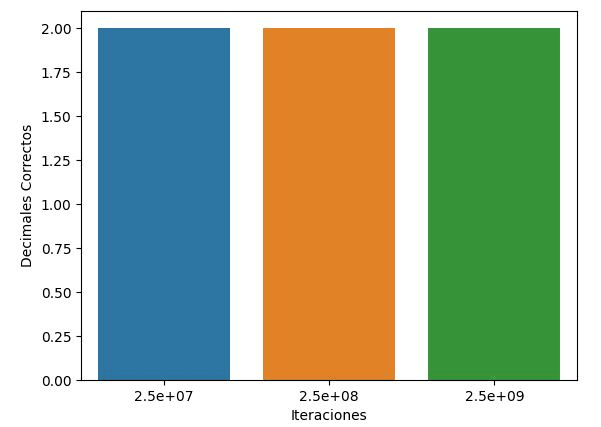
\includegraphics[width=100mm]{Figure_1.png}
    \caption{Diagrama decimal.}
    \label{figure}
\end{figure}
 \begin{subfigure}{1.1\textwidth}
         \centering
         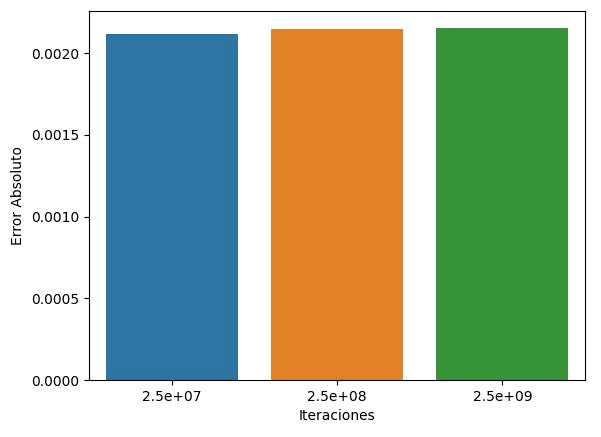
\includegraphics[width=100mm]{Figure_2.png}
         \caption{Diagrama Error.}
         \label{fig:tocan}
     \end{subfigure}
     \caption{Semillas de grietas de mayor valor.}
     \label{grietas}
\end{figure}

\begin{figure}
    \centering
    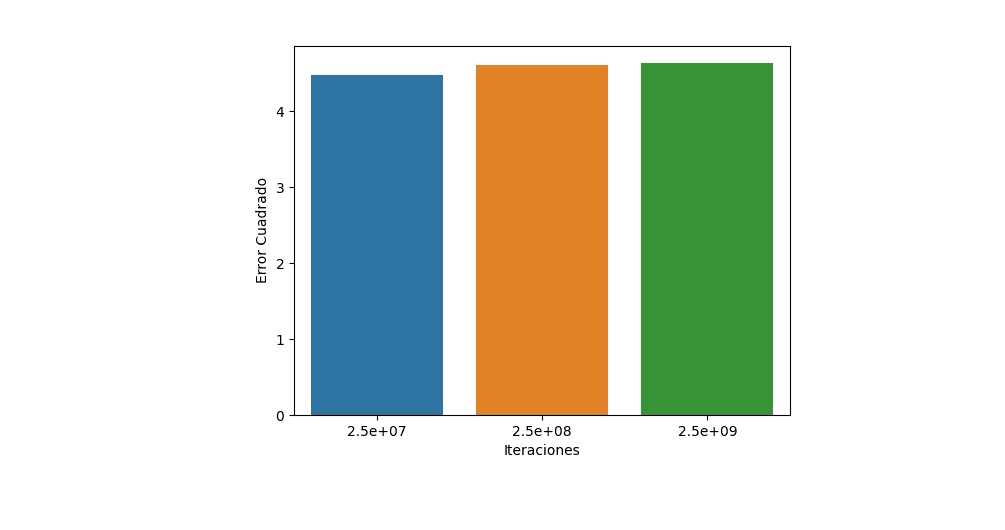
\includegraphics[width=90mm]{Figure_3.png}
    \caption{Diagrama Absoluto.}
    \label{figure}
\end{figure}


\section{Conclusiones}
Se concluye que las iteraciones representa una ligera variación va aumentando con respecto a la cantidad de iteraciones. Sin embargo cuando varía esto puede cambiar los valores para ser exactos debido a la ejecución.


\bibliographystyle{plainnat}
\cite{1}
\cite{2}
\cite{Matpltlib}
\bibliography{simulacion}

\end{document}
